\chapter{Projeto de Controlador com Alocação de Polos Baseado nos Modelos Identificados} \label{cap5}
Com o sistema identificado, podemos finalmente controlá-lo. Faremos isso através de realimentação de estados para os quatro modelos identificados.

\section{Alocação de Polos com Realimentação de Estados} \label{s:ctrl}
Para fazer o controle por realimentação de estados, precisamos passar os 3 modelos ARX obtidos para modelos em espaço de estados. Fazemos isso usando a função do Matlab tf2ss, onde entramos com o nominador e denominador do modelo ARX e a função nos retorna as matrizes A, B, C e D do sistema em espaço de estados. 


Queremos controlar os 4 modelos fazendo alocação de polos através da realimentação de estados. Projetamos os controladores para que atendam como requisitos um sobrevalor menor que 4\% do valor final e tempo de assentamento menor que 2 segundos quando recebe uma entrada do tipo degrau unitário.

\subsection{Modelo $SUB1$}\label{s:ctrlsub1}

Para atender os requisitos de tempo de assentamento $t_s<2 ~s$ e sobrevalor máximo de $ovs<4\%$ calculamos os valores de $\zeta$ e $\omega_n$ usados na equação característica de um sistema de segunda ordem \eqref{eq:mso}, usando as equações \eqref{eq:ovs} e \eqref{eq:ts}.

\begin{equation}\label{eq:mso}
G(s)=\dfrac{\omega_n^2}{s^2+2 \zeta \omega_n  s+ \omega_n^2}
\end{equation}

\begin{equation}\label{eq:ovs}
ovs=e^{\dfrac{\zeta \pi}{\sqrt{1-\zeta^2}}}<4\%
\end{equation}

\begin{equation}\label{eq:ts}
t_s=\dfrac{4}{\zeta \omega_n}<2~s
\end{equation}

Encontramos $\zeta>0.7157$ e $\omega_n>2.7945$, e escolhemos os valores de $\zeta=0.9$ e $\omega_n=4$. Ao aplicar esses valores na equação \eqref{eq:mso} obtivemos os polos que precisávamos alocar no domínio s, $s_1=-3.6000 + 1.7436i$ e $s_2=-3.6000 - 1.7436i$. Como o modelo $SUB1$ tem ordem 3, precisamos de um terceiro polo distante da parte real dos anteriores. Escolhemos $s_3=-8$. Passamos os três polos para o domínio z e obtivemos $z_1=0.8321 + 0.0727i$, $z_2=0.8321 - 0.0727i$ e $z_3=0.6703$. 


Para fazer a alocação de polos, usamos a equação de Lyapunov
\eqref{eq:lyapeq}:
\begin{equation}\label{eq:lyapeq}
(A-B\bar{k})T=TF
\end{equation}

Onde $A$ e $B$ são matrizes do sistema, $\bar{k}$ é um vetor arbitrário escolhido de forma que o par $F$ e $\bar{k}$ seja observável, $F$ é uma matriz em blocos diagonais com os polos que se deseja alocar e $k=\bar{k}*T^{-1}$ nos retorna o vetor de realimentação de estados $k$. Obtemos $k=[0.7552,~0.2637,~0.1750]$. Com essa realimentação de estados, obtivemos a seguinte resposta ao degrau:

\begin{figure}[H]
	\centering
	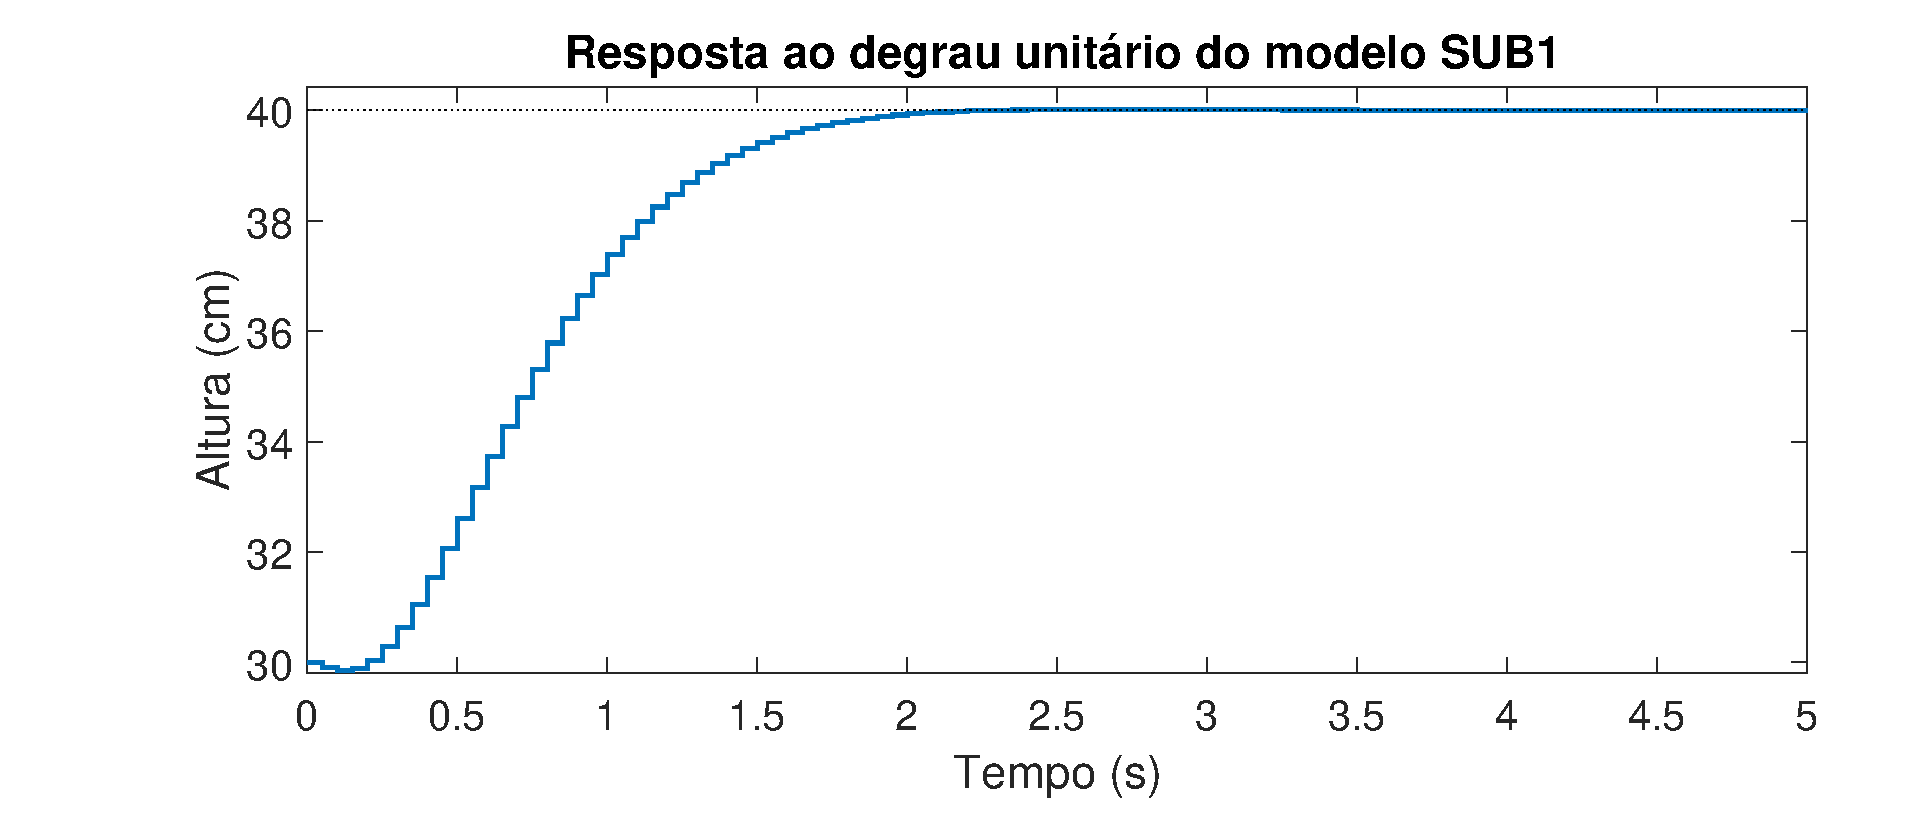
\includegraphics[width=1\linewidth]{respostadegrausub1c}
	\caption[Resposta ao degrau unitário do modelo $SUB1$ controlado]{Resposta ao degrau unitário do modelo simulado $SUB1$ controlado}
	\label{fig:respostadegrausub1c}
\end{figure}


A resposta ao degrau do sistema, como vista na figura \ref{fig:respostadegrausub1c}, apresentou um tempo de assentamento de 1.8 segundos e um sobrevalor de 0.14\%.

\subsection{Modelo $ARX1$}\label{s:ctrlarx1}

Para o modelo $ARX1$, escolhemos os valores de $\zeta=0.9$ e $\omega_n=7$. Ao aplicar esses valores na equação \eqref{eq:mso}, obtivemos os polos que precisamos alocar no domínio s, $s_1=-6.3000 + 3.0512i$ e $s_2=-6.3000 - 3.0512i$, para o polo distante alocamos $s_3=-15$. Que no domínio z são $z_1=0.7213 + 0.1109i$, $z_2=0.7213 - 0.1109i$ e $z_3=0.4966$. Repetimos o mesmo procedimento de alocação de polos usado no modelo $SUB1$ e obtivemos $k=[-0.2840,~0.6313,~-0.3481]$.


O sistema realimentado teve a seguinte resposta ao degrau:

\begin{figure}[H]
	\centering
	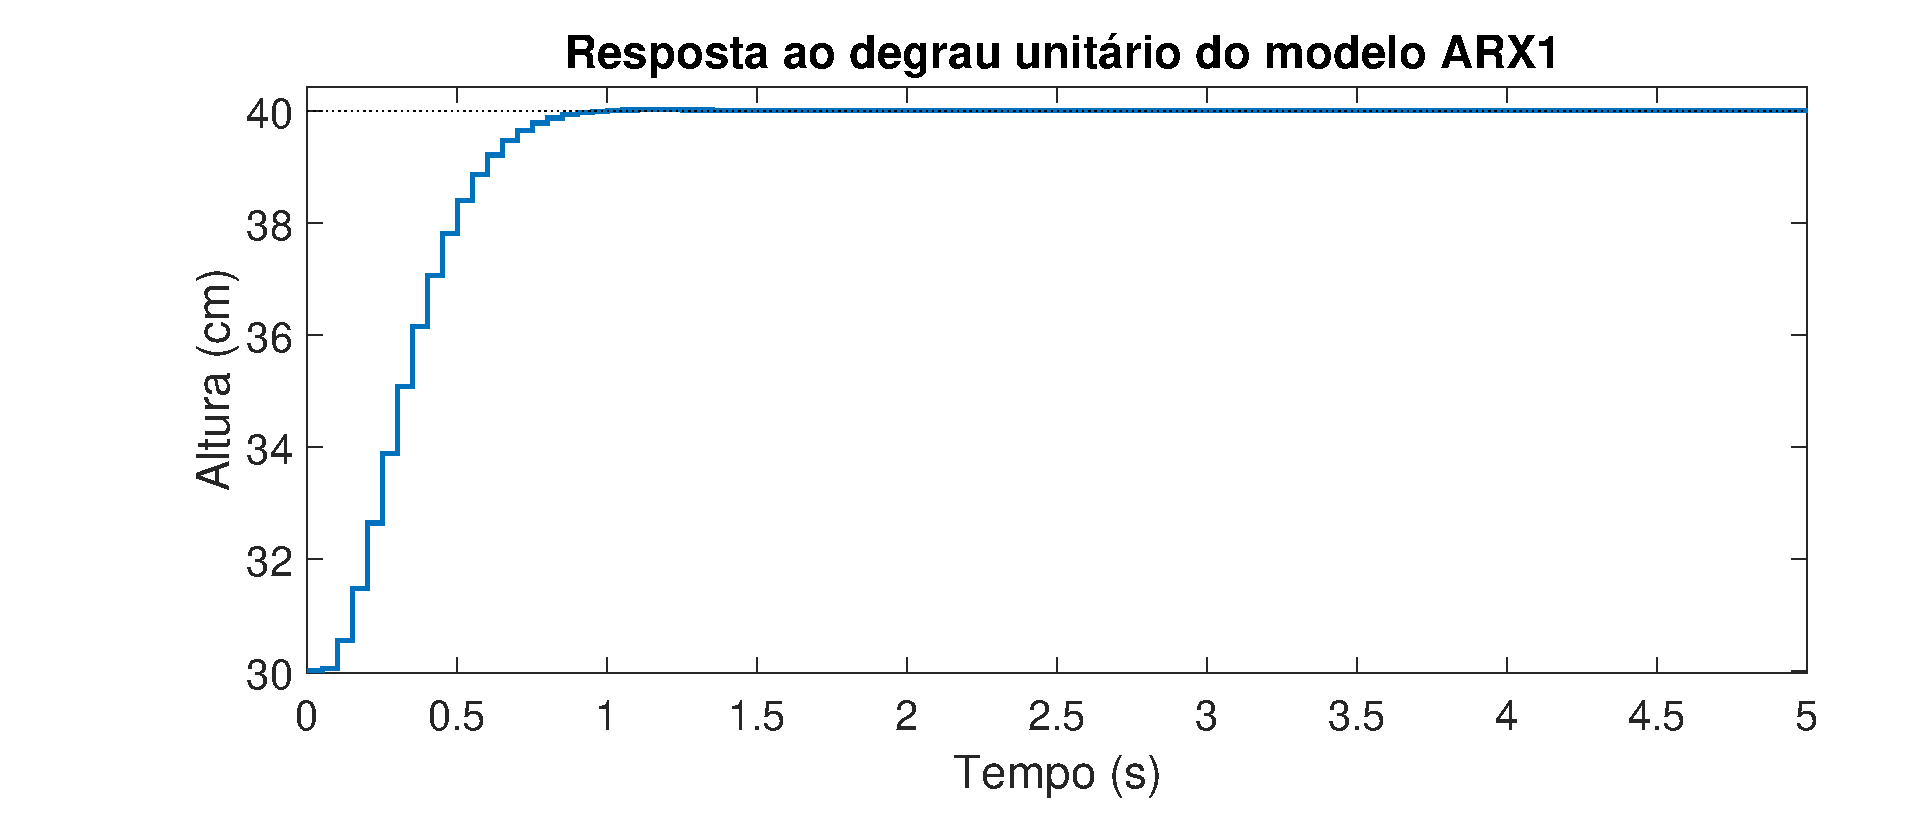
\includegraphics[width=1\linewidth]{respostadegrauarx1c}
	\caption[Resposta ao degrau do modelo simulado $ARX1$ controlado]{Resposta ao degrau do modelo simulado $ARX1$ controlado}
	\label{fig:respostadegrauarx1c}
\end{figure}


A resposta ao degrau da figura \ref{fig:respostadegrauarx1c} apresenta um tempo de assentamento de 0.8 segundos e um sobrevalor de 0,125\%.

\subsection{Modelo $ARX2$}\label{s:ctrlarx2}
Para o modelo $ARX2$, escolhemos $\zeta=0.9$ e $\omega_n=9$. Aplicando na equação \eqref{eq:mso} obtivemos os polos para alocar no domínio s, $s_1=-8.1000 + 3.9230i$ e $s_2=-8.1000 - 3.9230i$. Este modelo ainda tem 3 polos extras que devem ser alocados distantes dos polos $s_1$ e $s_2$, escolhemos $s_3=-14$, $s4=-14.1$ e $s_5=-14.2$. Que no domínio z são $z_1=0.6542 + 0.1300i$, $z_2=0.6542 - 0.1300i$, $z_3=0.4966$, $z_4=0.4941$ e $z_5=0.4916$. Fazendo a alocaçao de polos da mesma forma que foi feita para o modelo $SUB1$, obtivemos $k=[-1.2401,~2.3566,~-1.2062,~-0.0018,~0.0360]$.

O sistema controlado teve a seguinte resposta ao degrau unitário:

\begin{figure}[H]
	\centering
	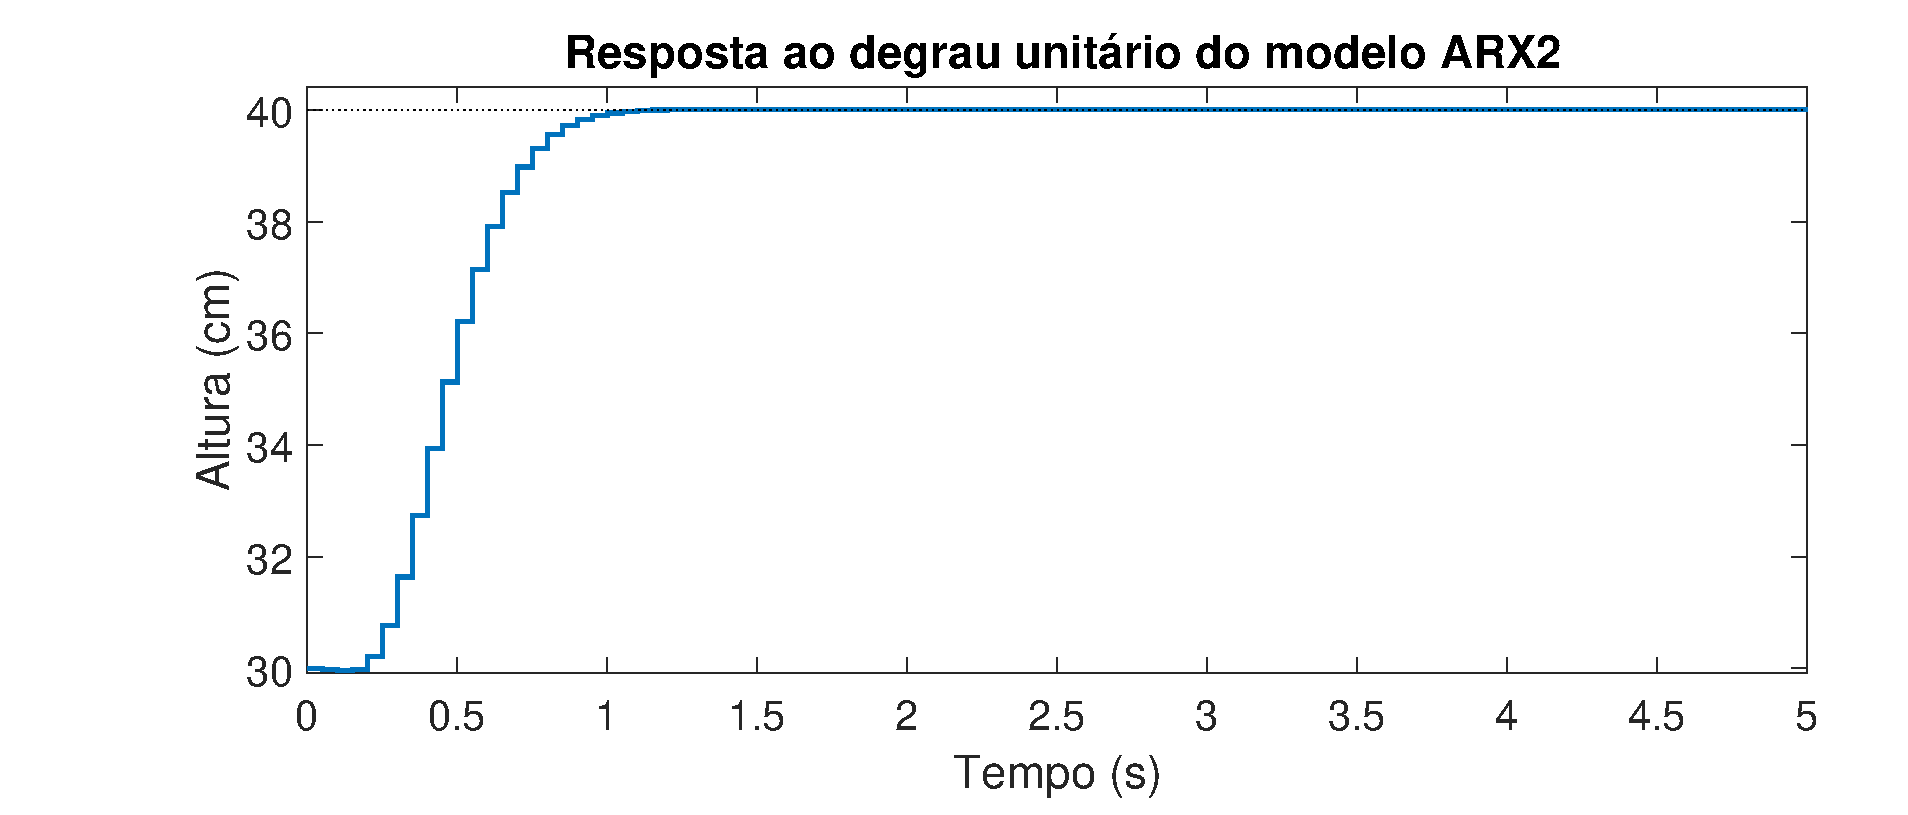
\includegraphics[width=1\linewidth]{respostadegrauarx2c}
	\caption[Resposta ao degrau do modelo $ARX2$]{Resposta ao degrau do modelo simulado $ARX2$ controlado}
	\label{fig:respostadegrauarx2c}
\end{figure}

Vemos na figura \ref{fig:respostadegrauarx2c}, que a resposta ao degrau unitário do sistema controlado teve tempo de assentamento de 0.9 segundos e sobrevalor de 0.0326\%.


\subsection{Modelo $ARXsim$}\label{s:ctrlarxsim}

Para o modelo $ARXsim$, escolhemos $\zeta=0.9$ e $\omega_n=9$. Aplicados na equação\eqref{eq:mso} obtivemos os polos no domínio s, $s_1=-3.6000 + 1.7436i$ e $s_2=-3.6000 - 1.7436i$, e escolhemos o polo distante $s_3=-8$. No domínio z os polos são $z_1=0.8321 + 0.0727i$, $z_2=0.8321 - 0.0727i$ e $z_3=0.4966$. Fizemos a alocação de polos como foi feito para o modelo $SUB1$ e obtivemos $k=[-1.1499,~1.0710,~0.0876]$.
O sistema controlado teve a seguinte resposta ao degrau unitário:

\begin{figure}[H]
	\centering
	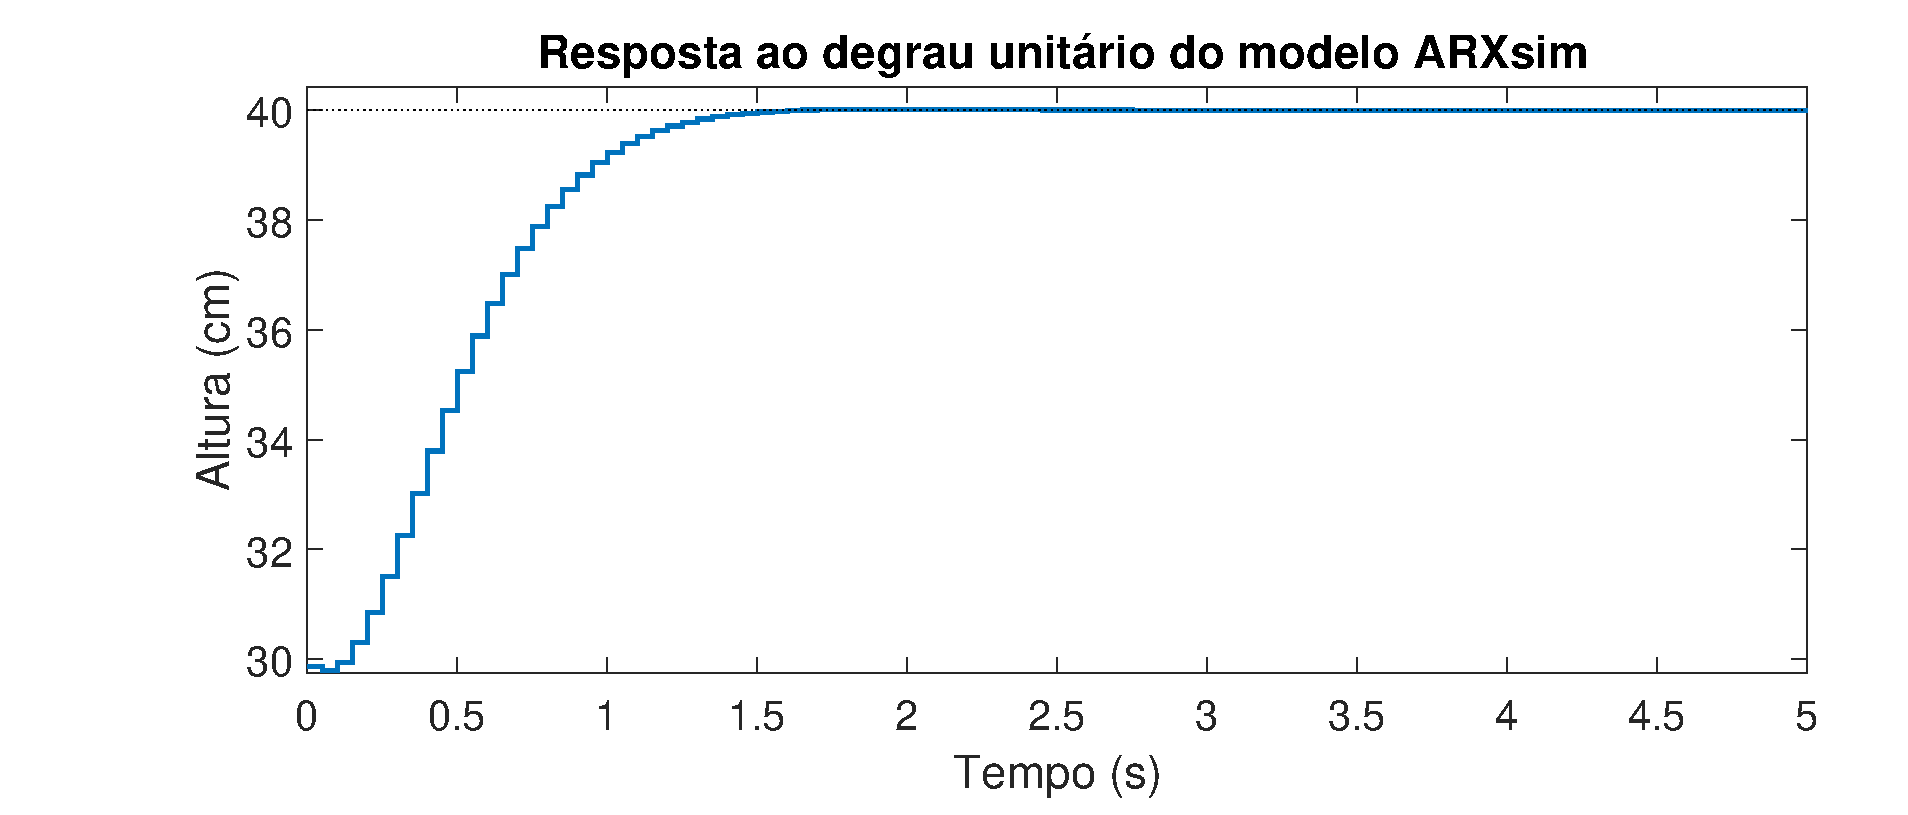
\includegraphics[width=1\linewidth]{respostadegrauarxsimc}
	\caption[Resposta ao degrau do modelo simulado $ARXsim$]{Resposta ao degrau do modelo simulado $ARXsim$ controlado}
	\label{fig:respostadegrauarxsimc}
\end{figure}

Vemos na figura \ref{fig:respostadegrauarxsimc}, que a resposta ao degrau unitário do sistema controlado teve tempo de assentamento de 1.3 segundos e máximo sobrevalor de 0.1487\%.


\section{Projeto do Estimador de Estados}\label{s5:est}
Para realizar um controlador por realimentação de estados, precisamos ser capazes de medir todos os estados do nosso modelo a cada tempo de amostragem. O nosso sistema, no entanto, não tem sensores para medir cada um dos estados necessários. A única medida disponível é a saída do sistema na forma da altura da bola. Portanto, precisamos implementar um estimador de estados para cada um dos controladores projetados na subseção anterior.

\subsection{Modelo $SUB1$}\label{s:estsub1}
Um estimador de estados é projetado de forma similar ao controlador por realimentação de estados, precisamos escolher polos adequados para que o estimador funcione da forma correta. A forma mais simples de escolher esses polos é fazer com que eles reajam mais rápido que o sistema à entrada recebida. Conseguimos isso, multiplicando a parte real dos polos no domínio s por um número para que fossem mais rápidos. 


Projetamos o estimador de estados com os seguintes polos $z_1=0.1647 + 0.0144i$, $z_2=0.1647 - 0.0144i$ e $z_3=0.0183$ e obtivemos o ganho do estimador $L=[3.5436,~-7.2192,~13.9077]^T$. Nas figuras \ref{fig:estimadorsub1} e \ref{fig:stepestsub1}, vemos como uma simulação do sistema se comportou.

\begin{figure}[H]
	\centering
	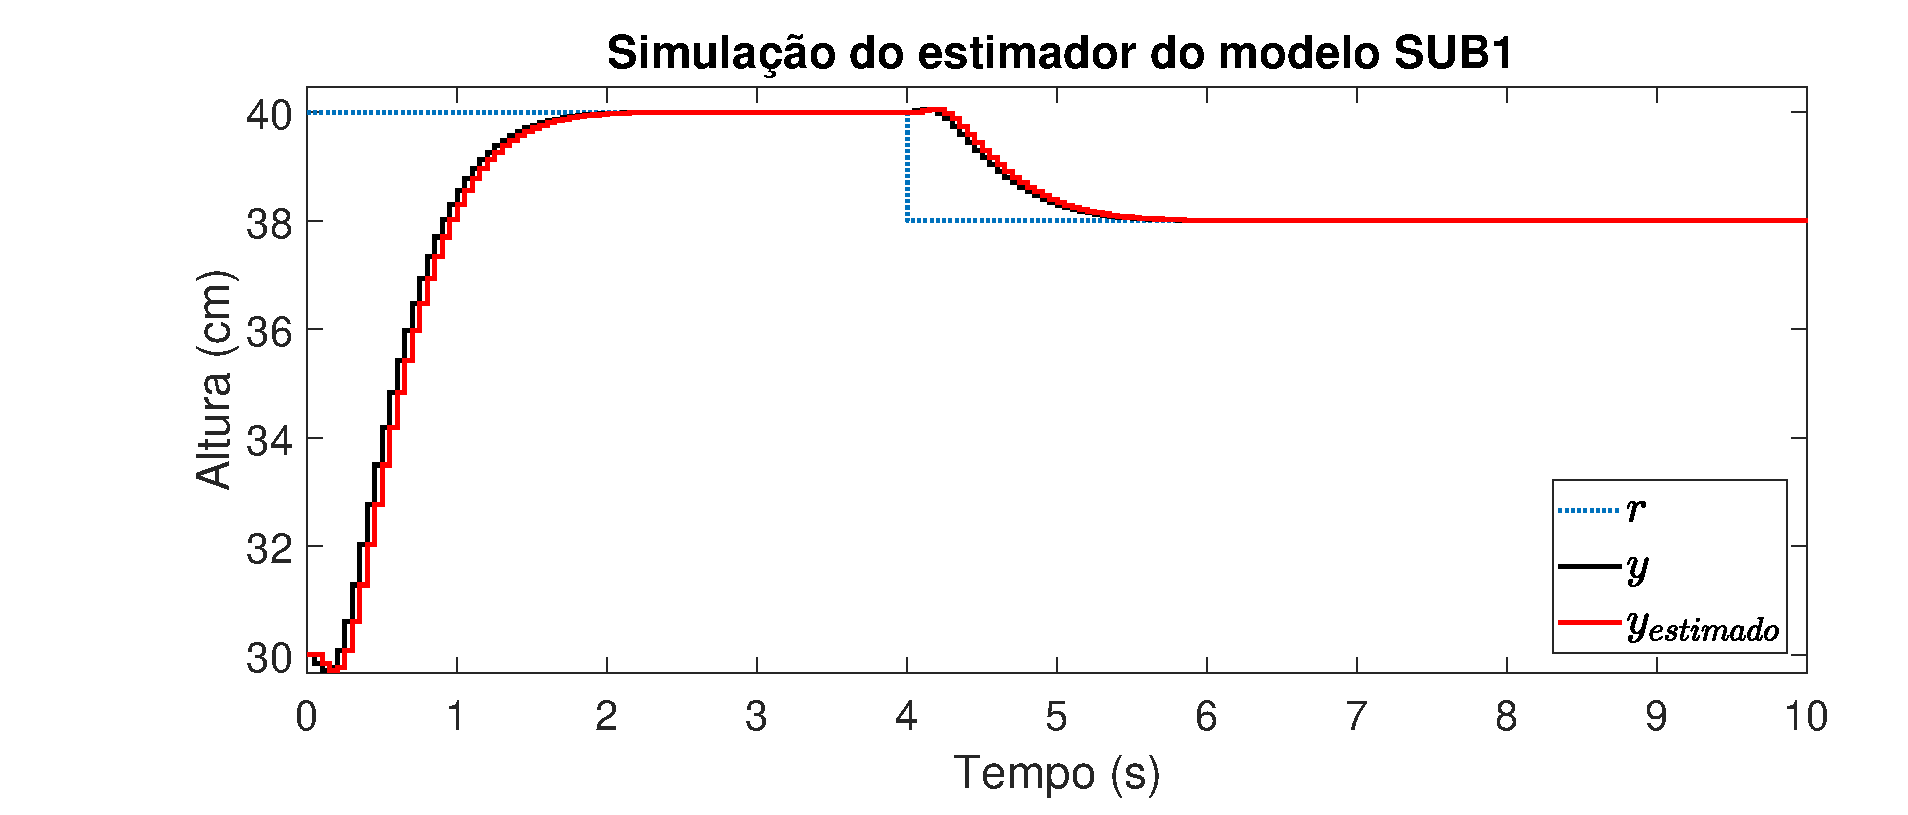
\includegraphics[width=1\linewidth]{estimadorsub1}
	\caption[Simulação do estimador do modelo $SUB1$]{Simulação do estimador do modelo $SUB1$}
	\label{fig:estimadorsub1}
\end{figure}

\begin{figure}[H]
	\centering
	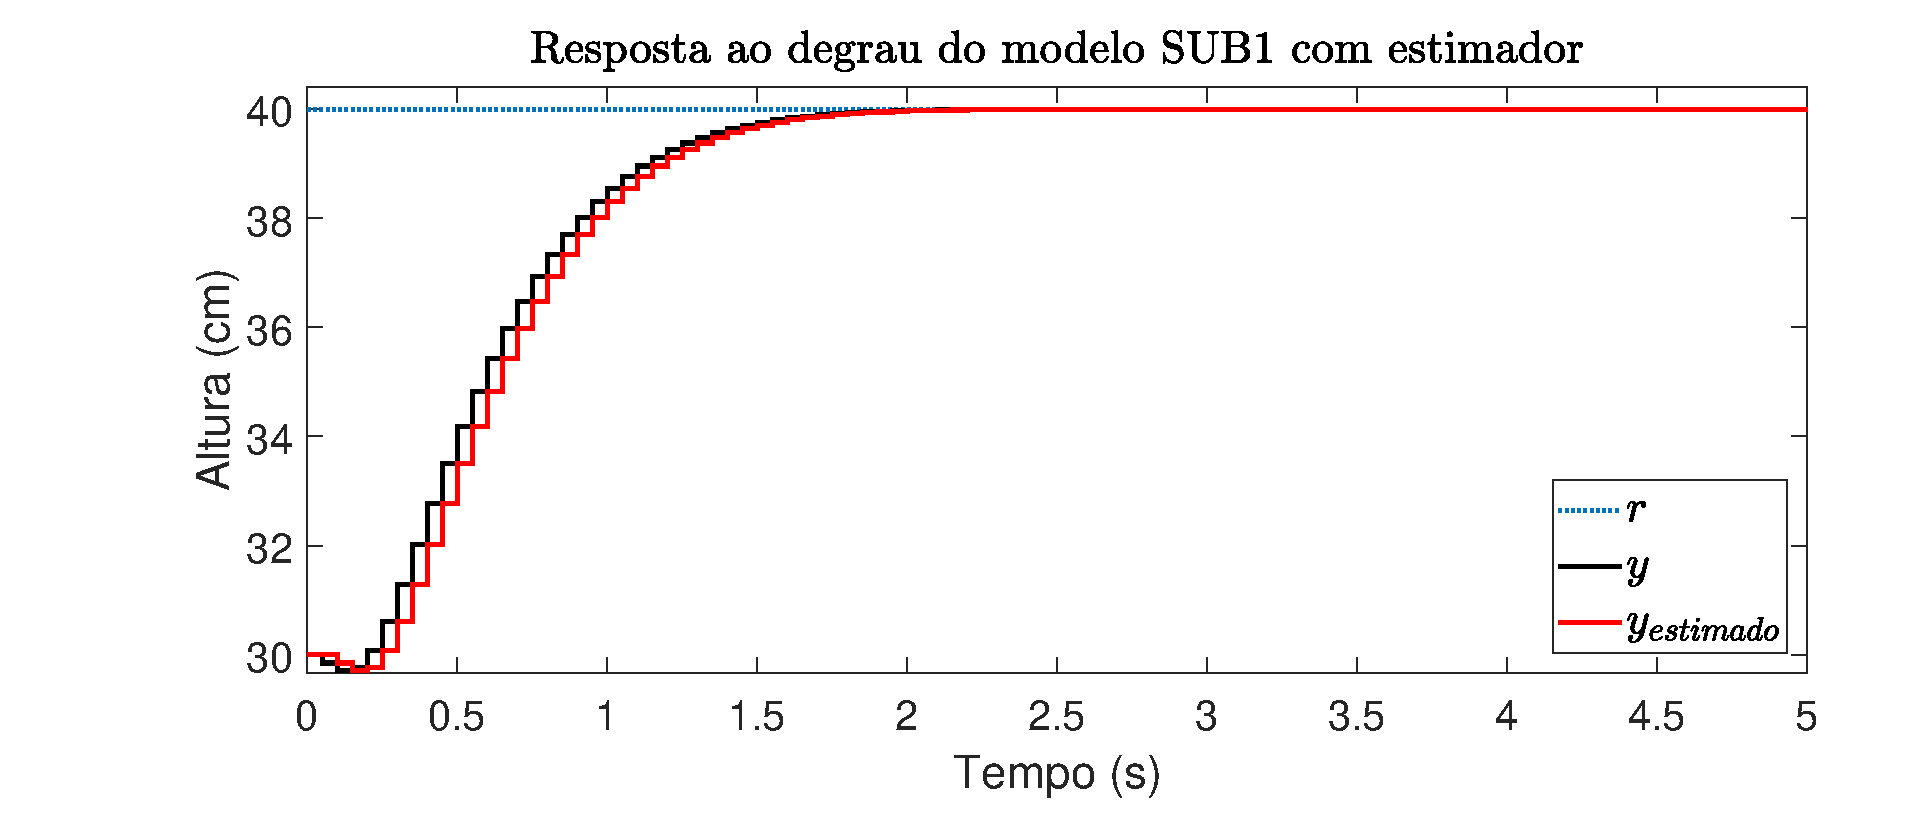
\includegraphics[width=1\linewidth]{stepestsub1}
	\caption[Resposta ao degrau do modelo $SUB1$ controlado com observador]{Resposta ao degrau do modelo $SUB1$ controlado com observador}
	\label{fig:stepestsub1}
\end{figure}



\subsection{Modelo $ARX1$}\label{s:estarx1}
Para o estimador do modelo $ARX1$, alocamos os polos em $z_1=0.0309 + 0.0048i$, $z_2=0.0309 - 0.0048i$ e $z_3=0.0003$. Obtivemos o ganho do estimador $L=[33.9534,~26.6709,~16.6024]^T$. Nas figuras \ref{fig:estimadorarx1} e \ref{fig:stepestarx1}, vemos como uma simulação do sistema se comportou.

\begin{figure}[H]
	\centering
	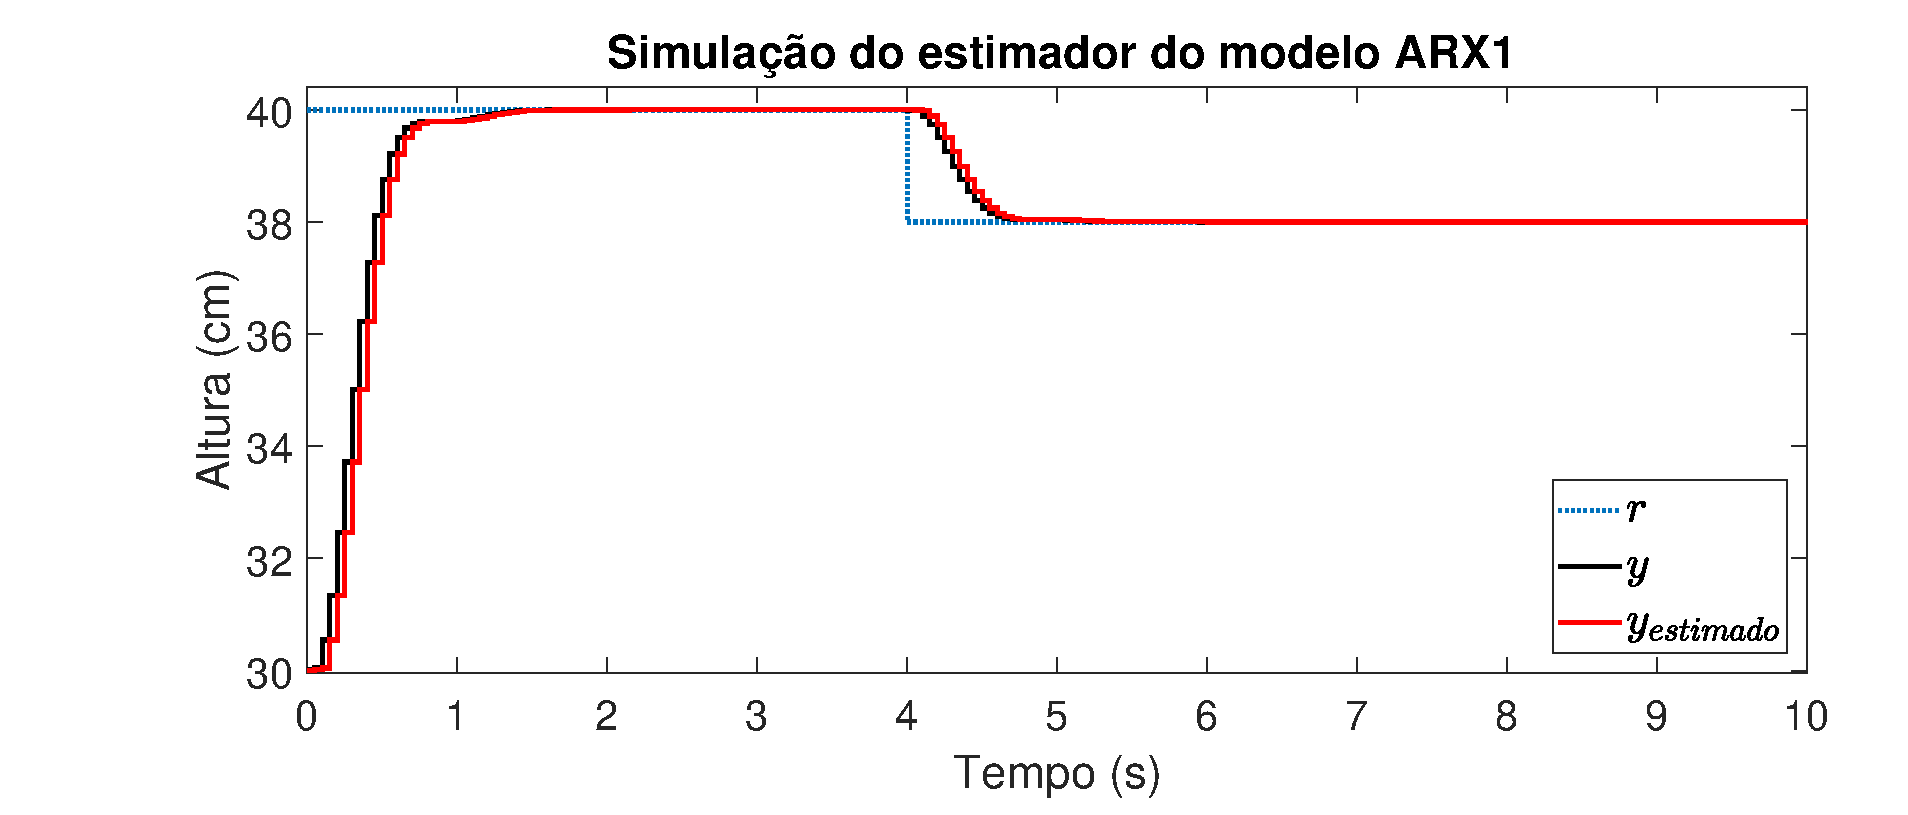
\includegraphics[width=1\linewidth]{estimadorarx1}
	\caption[Simulação do estimador do modelo $ARX1$]{Simulação do estimador do modelo $ARX1$}
	\label{fig:estimadorarx1}
\end{figure}

\begin{figure}[H]
	\centering
	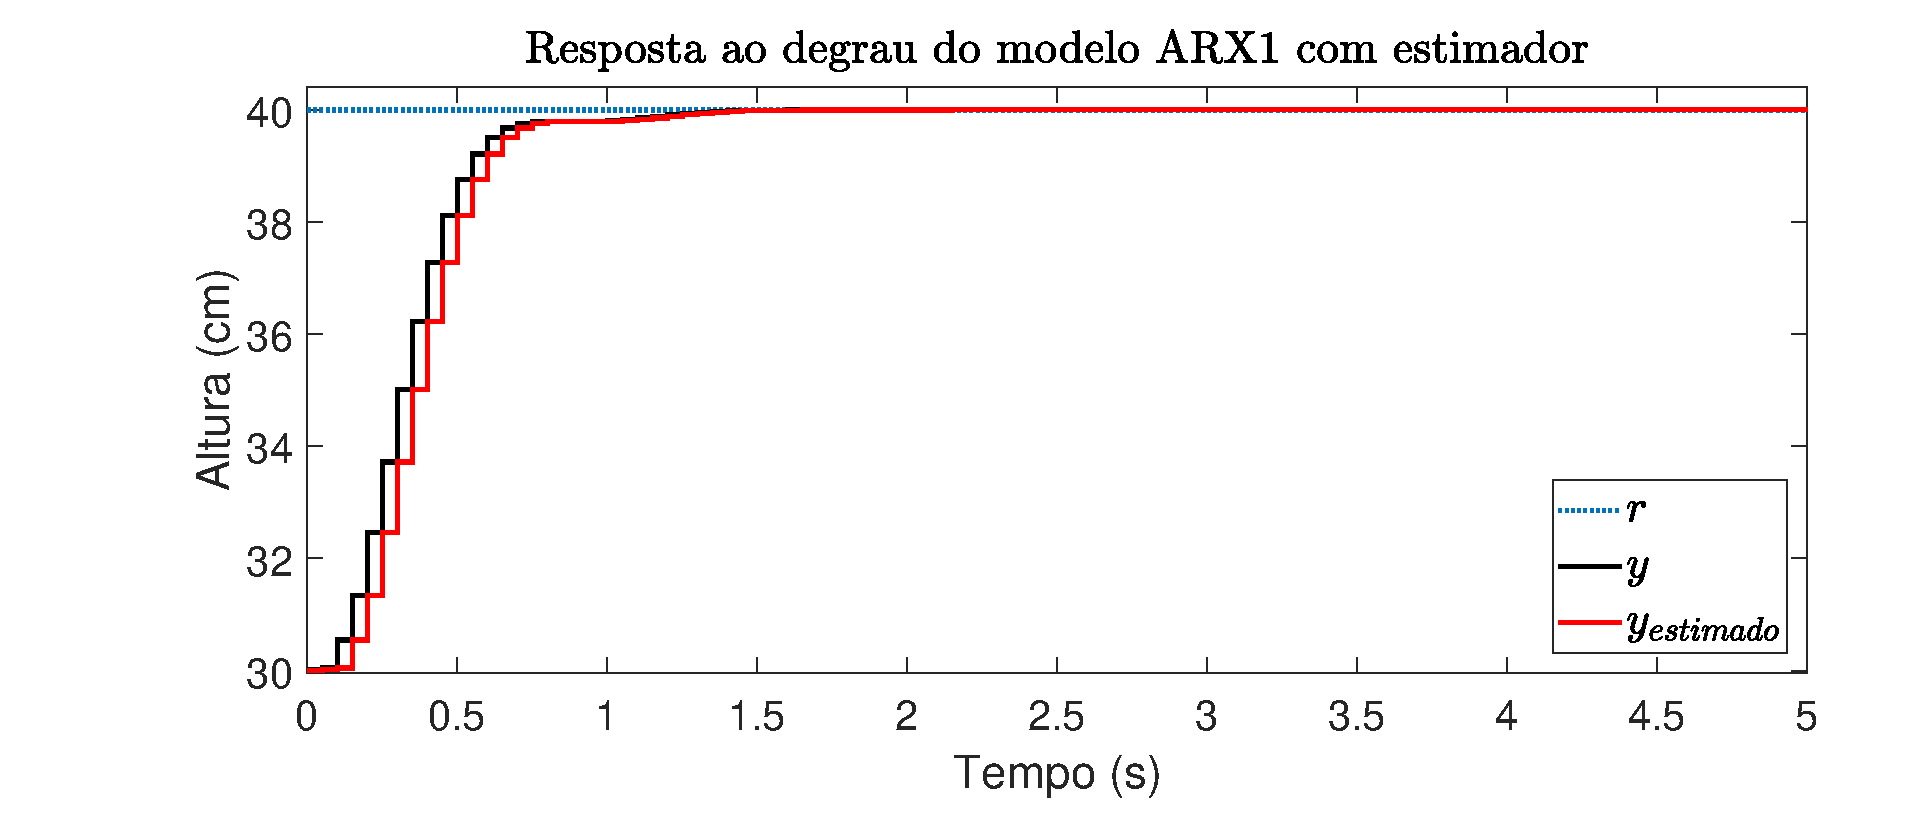
\includegraphics[width=1\linewidth]{stepestarx1}
	\caption[Resposta ao degrau do modelo $ARX1$ controlado com observador]{Resposta ao degrau do modelo $ARX1$ controlado com observador}
	\label{fig:stepestarx1}
\end{figure}

\subsection{Modelo $ARX2$}\label{s:estarx2}
Para o estimador do modelo $ARX2$, alocamos os polos em $z_1=0.0304 + 0.0074i$, $z_2=0.0304 - 0.0074i$, $z_3=0.0074$, $z_4=0.0072$ e $z_5=0.0069$. Obtivemos o ganho do estimador $L=[22.1925,~20.4118,~ 16.9038,~16.9671,~11.1584]^T$. Nas figuras \ref{fig:estimadorarx2} e \ref{fig:stepestarx2}, vemos como uma simulação do sistema se comportou.

\begin{figure}[H]
	\centering
	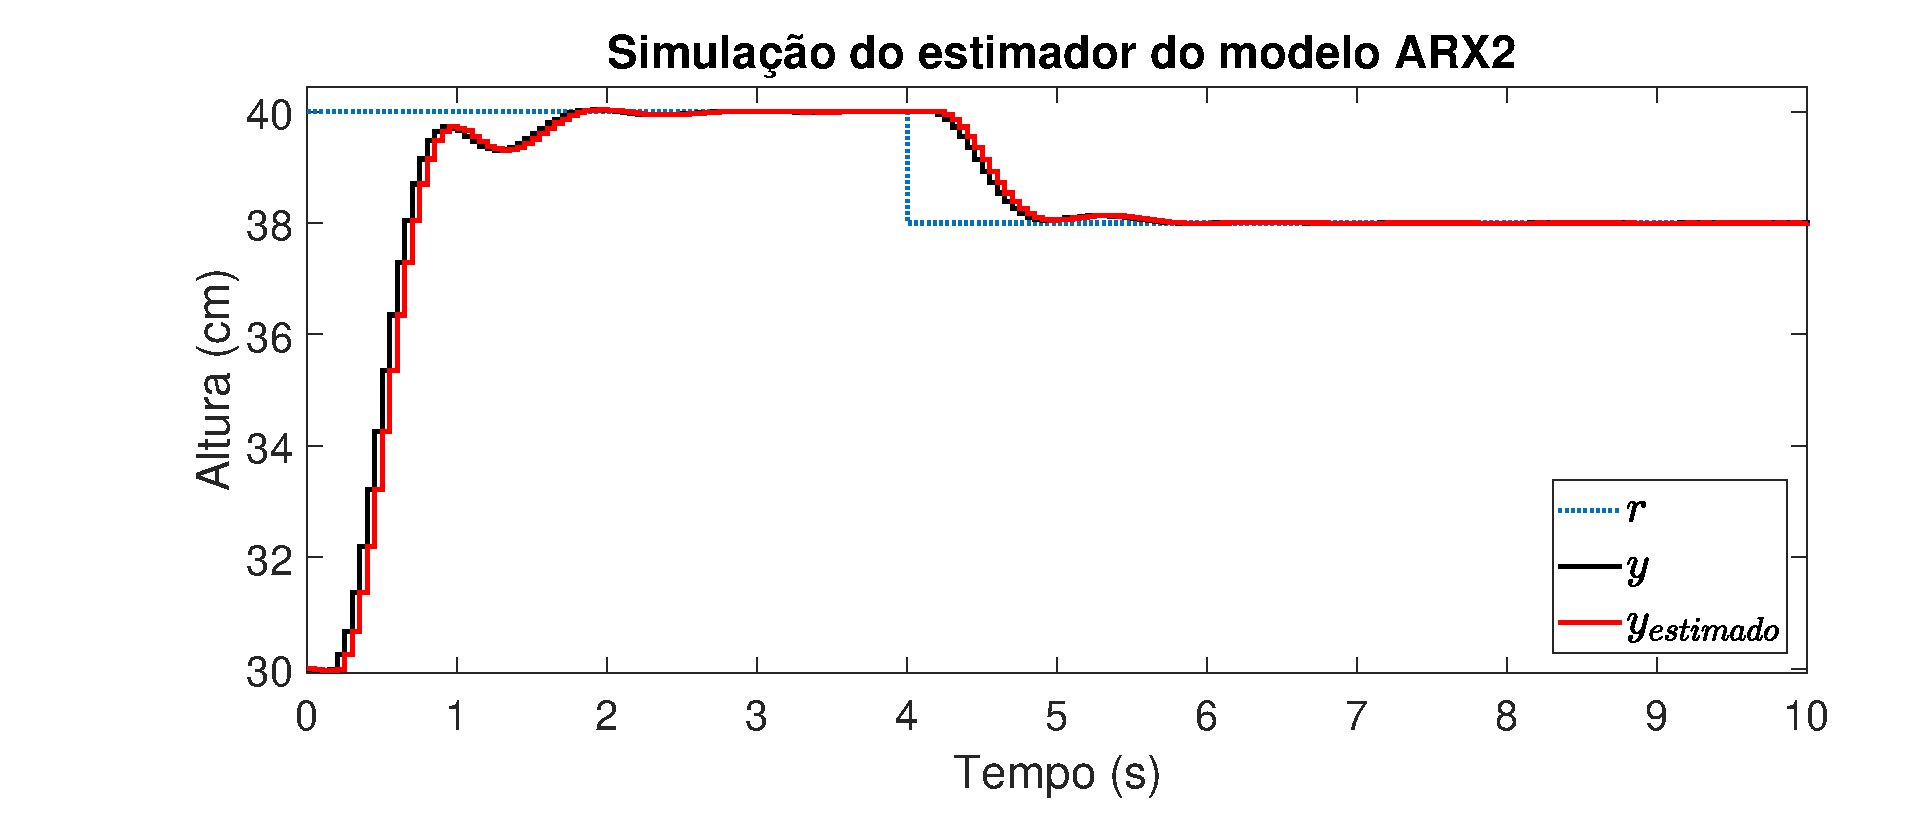
\includegraphics[width=1\linewidth]{estimadorarx2}
	\caption[Simulação do estimador do modelo $ARX2$]{Simulação do estimador do modelo $ARX2$}
	\label{fig:estimadorarx2}
\end{figure}

\begin{figure}[H]
	\centering
	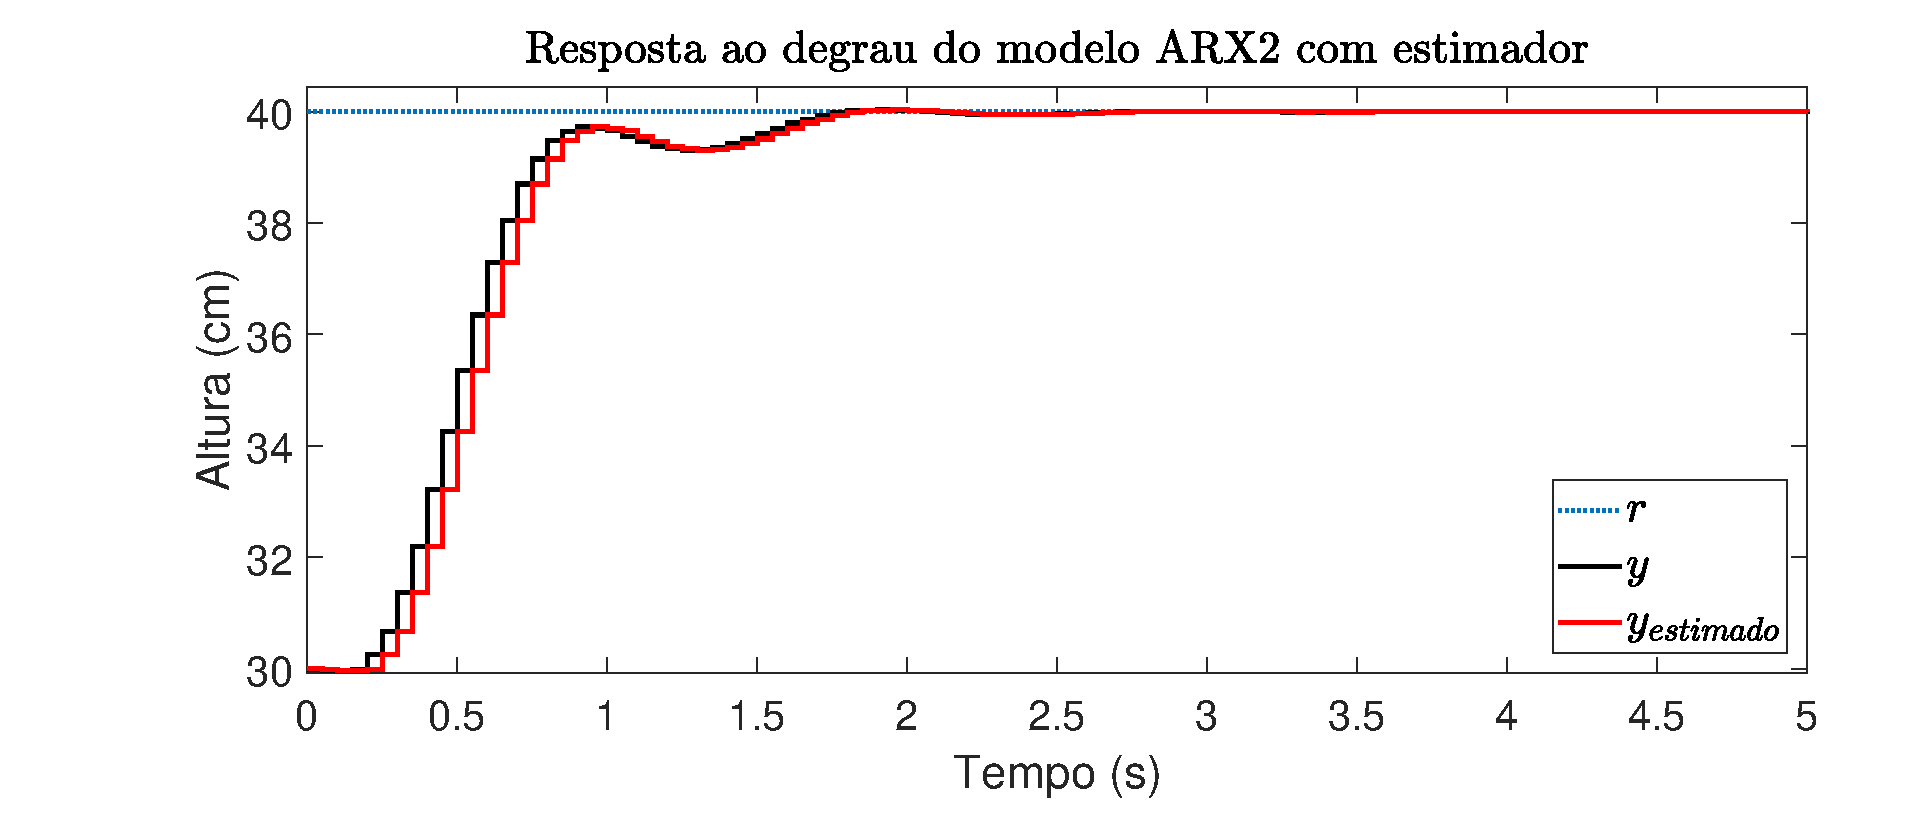
\includegraphics[width=1\linewidth]{stepestarx2}
	\caption[Resposta ao degrau do modelo $ARX2$ controlado com observador]{Resposta ao degrau do modelo $ARX2$ controlado com observador}
	\label{fig:stepestarx2}
\end{figure}

\subsection{Modelo $ARXsim$}\label{s:estarxsim}
Para o estimador do modelo $ARX2$, alocamos os polos em $z_1=0.3383 + 0.0296i$, $z_2=0.3383 - 0.0296i$ e $z_3=0.0150$. Obtivemos o ganho do estimador $L=[27.5247,~ 73.1490,~ 146.4144]^T$. Nas figuras \ref{fig:estimadorarxsim} e \ref{fig:stepestarxsim}, vemos como uma simulação do sistema se comportou.

\begin{figure}[H]
	\centering
	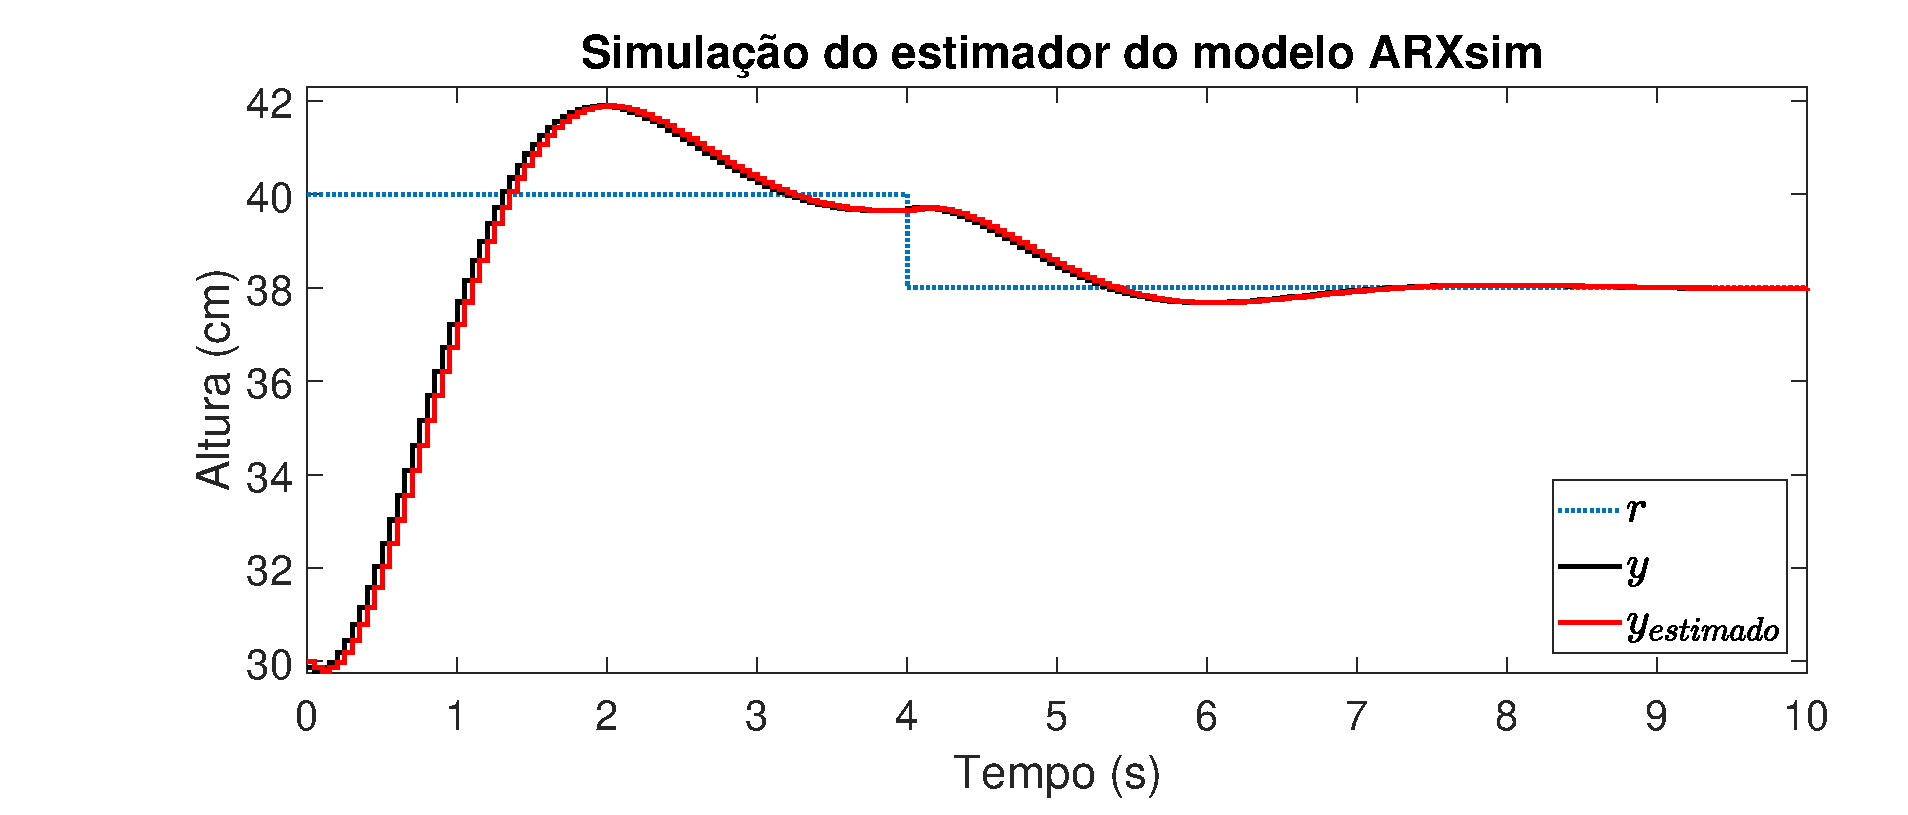
\includegraphics[width=1\linewidth]{estimadorarxsim}
	\caption[Simulação do estimador do modelo $ARXsim$]{Simulação do estimador do modelo $ARXsim$}
	\label{fig:estimadorarxsim}
\end{figure}

\begin{figure}[H]
	\centering
	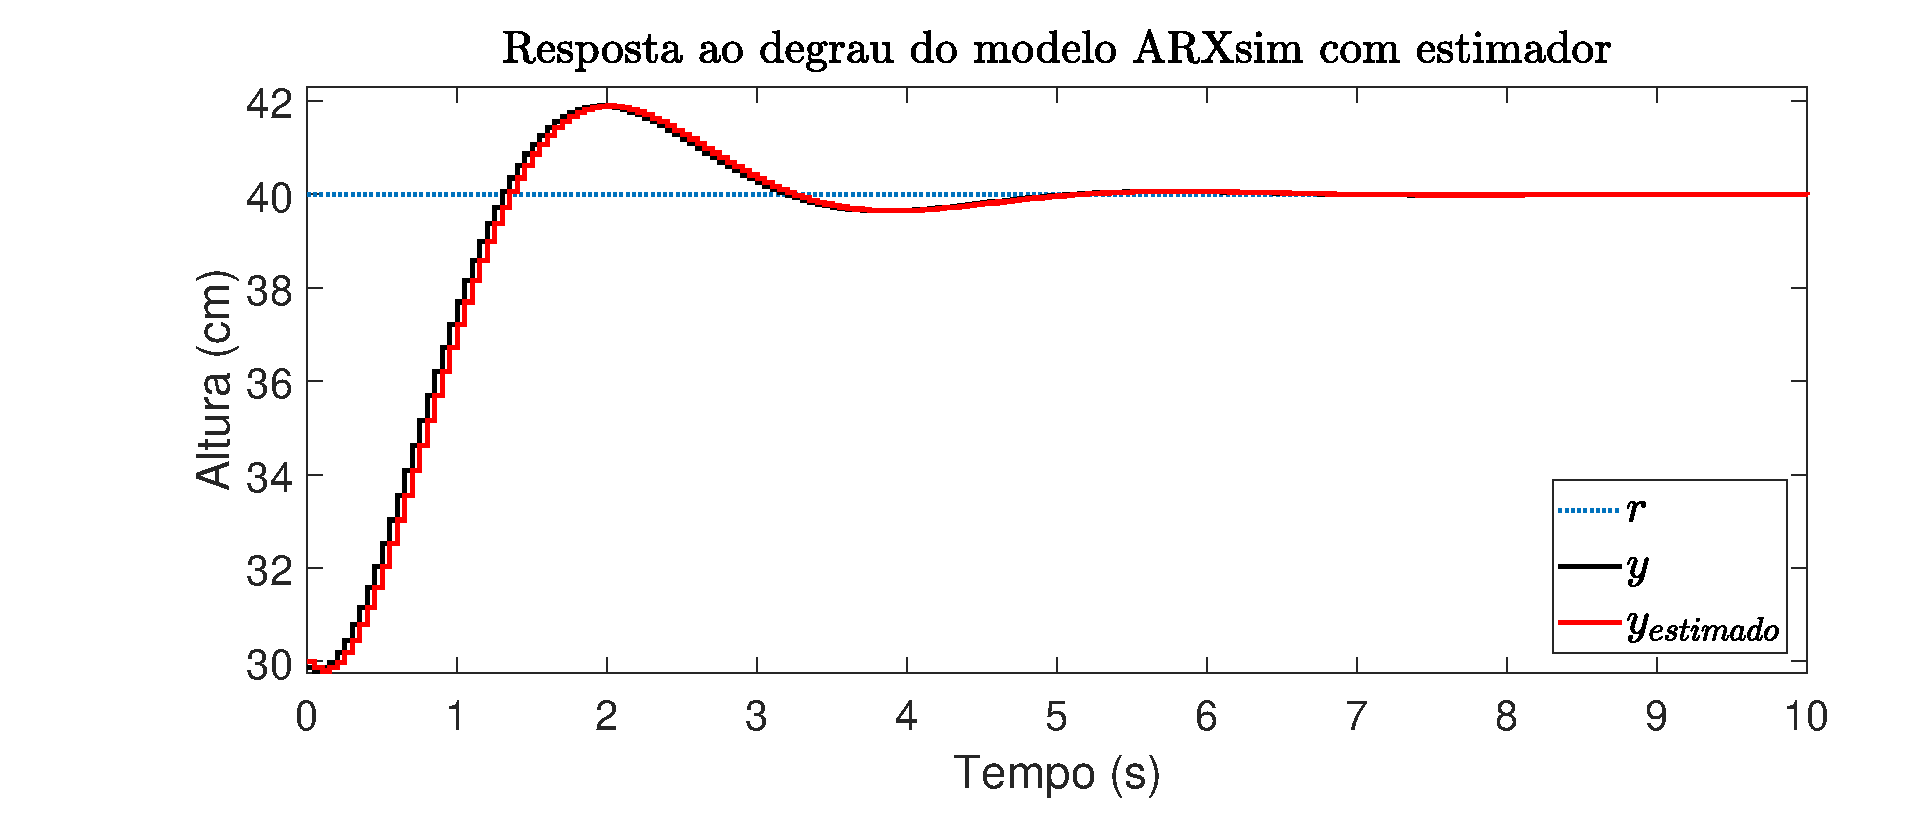
\includegraphics[width=1\linewidth]{stepestarxsim}
	\caption[Resposta ao degrau do modelo $ARXsim$ controlado com observador]{Resposta ao degrau do modelo $ARXsim$ controlado com observador}
	\label{fig:stepestarxsim}
\end{figure}














% Fim Capítulo
